\subsection{Baseline}
\begin{figure}[h]
	\centering
	\begin{subfigure}{0.48\linewidth}
		\centering
		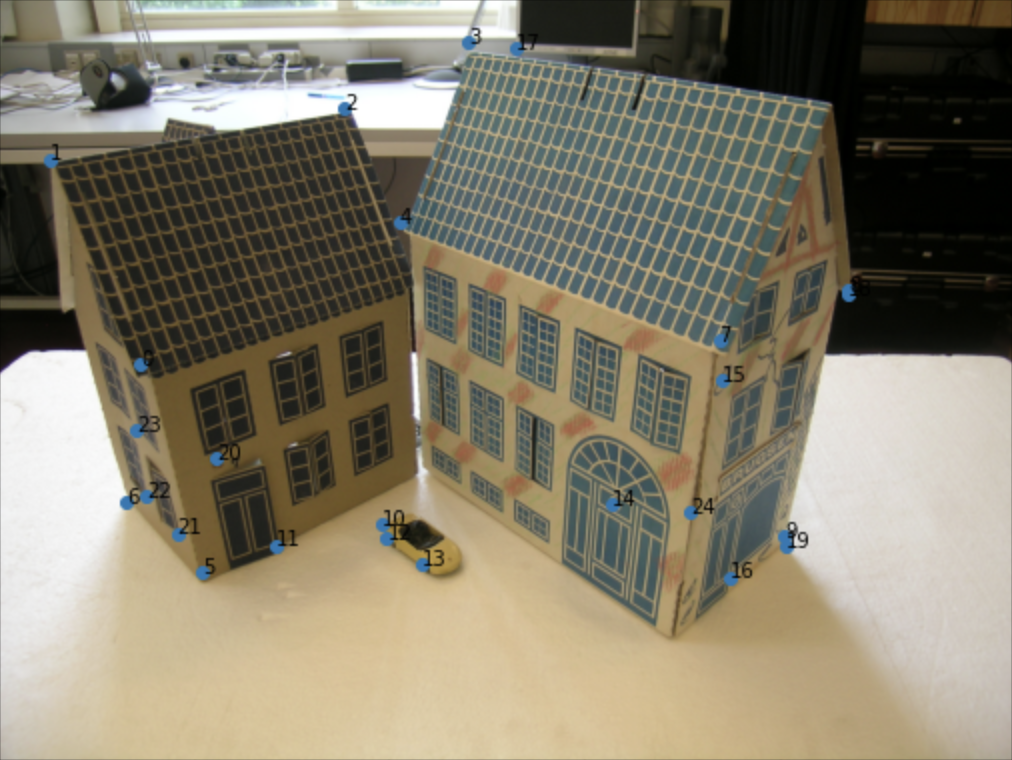
\includegraphics[width=\linewidth]{Materials/BaselineA}
	\end{subfigure}
	\hfill
	\begin{subfigure}{0.48\linewidth}
		\centering
		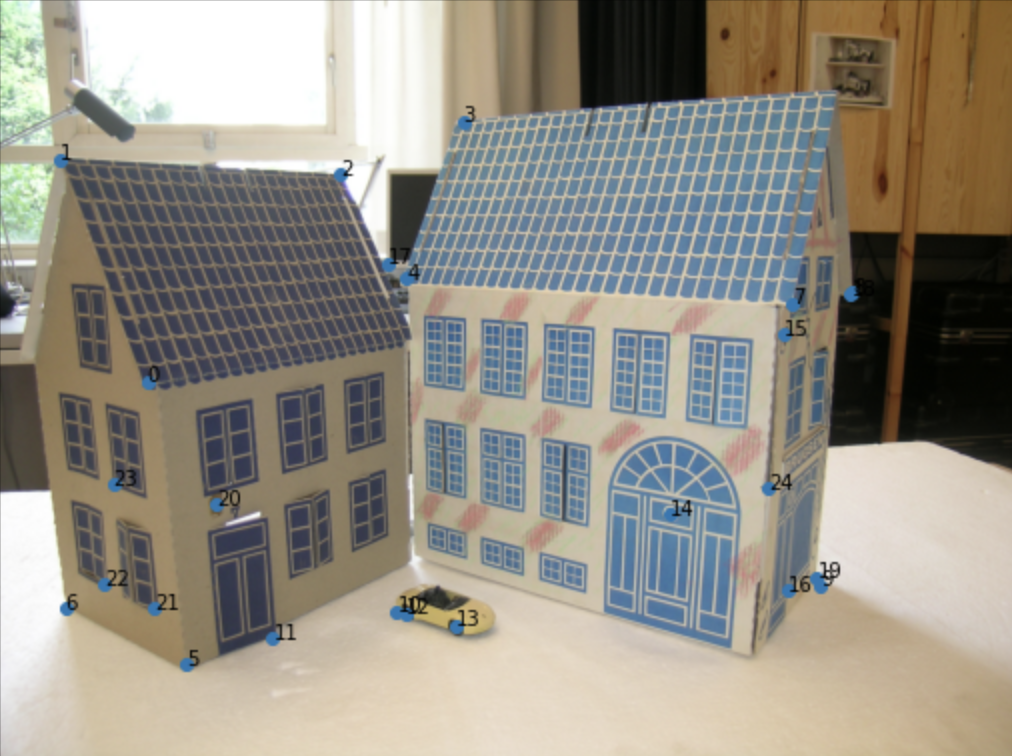
\includegraphics[width=\linewidth]{Materials/BaselineB}
	\end{subfigure}
	\caption{The 25 point correspondences between the two images found.}
	\label{correspondences}
\end{figure}
We will begin by establishing a baseline for comparison with the following experiments. This baseline will be the most naive / simple solution to estimating the fundamental matrix and bring the two images to scanline agreement. We begin by manually estimating 25 point correspondences between the two images which can be seen in \autoref{correspondences}. We now normalize the points found in each image separately by subtracting the mean of the points and dividing with their standard deviation. This gives us $T_A$ and $T_B$ which are transformation matrices for image A (left) and image B (right), and we will use these to denormalize the fundamental after its estimation. We can now estimate the (denormalized) fundamental matrix using the 8-point algorithm and report it to be:
\begin{equation*}
	F = \begin{bmatrix}
		1.08e-07 & 8.30e-08 & 6.90e-04\\
		-1.27e-07 & -1.11e-07 & 9.40e-04\\
		-9.15e-04 &-7.49e-04 & -4.59e-02
	\end{bmatrix}
\end{equation*}
With the fundamental matrix we can now use \textit{opencv} to find the epipolar lines and draw them on the images, as done in \autoref{baselineepipolarlines}.
\begin{figure}[h]
	\centering
	\begin{subfigure}{0.48\linewidth}
		\centering
		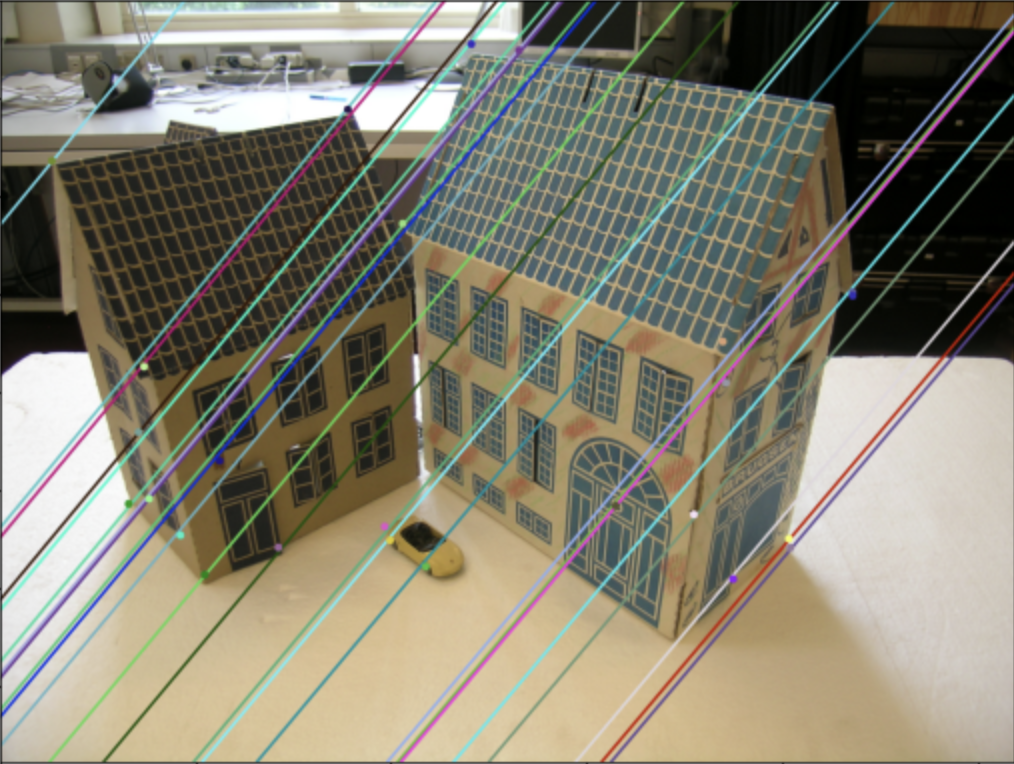
\includegraphics[width=\linewidth]{Materials/BaselineEpiA}
	\end{subfigure}
	\hfill
	\begin{subfigure}{0.48\linewidth}
		\centering
		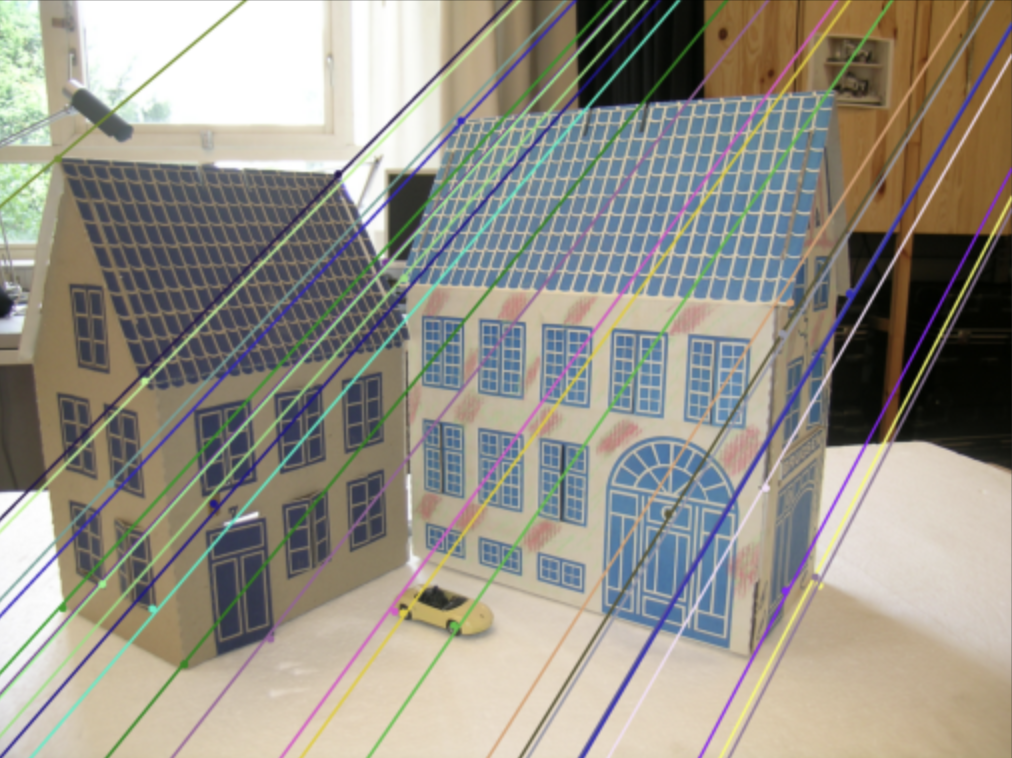
\includegraphics[width=\linewidth]{Materials/BaselineEpiB}
	\end{subfigure}
	\caption{Epipolar lines drawn on top of the two images.}
	\label{baselineepipolarlines}
\end{figure}
By computing the left and right null vectors of the fundamental matrix, $F$, we can get the coordinates of the epipoles. We find the left epipole, i.e. the optical center of the right camera projected into the left cameras view, to be at coordinates $[-104610.58, 127733.71]$, and the right epipole, i.e. the optical center of the left camera projected into the right cameras view, to be $[4577.86, -3312.85]$.\\
We can now bring the two images to scanline agreement using \textit{opencv} which can be seen in \autoref{baselineScanline}.
\begin{figure}[h]
	\centering
	\begin{subfigure}{0.48\linewidth}
		\centering
		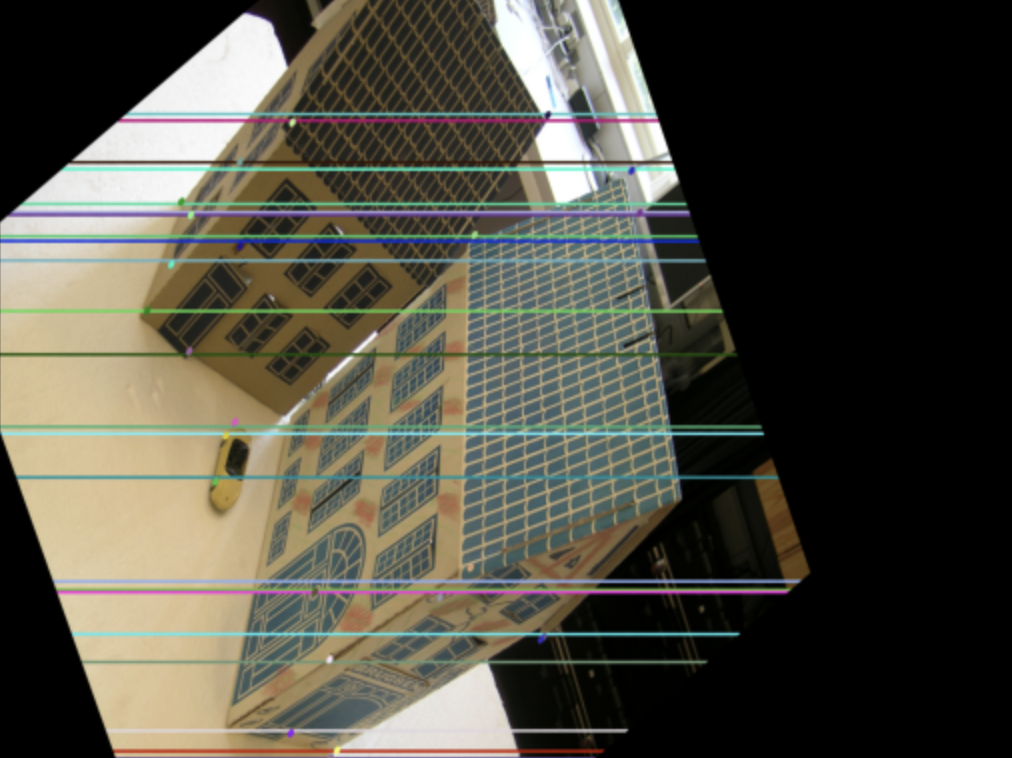
\includegraphics[width=\linewidth]{Materials/BaselineScanlineA}
	\end{subfigure}
	%\hfill
	\begin{subfigure}{0.48\linewidth}
		\centering
		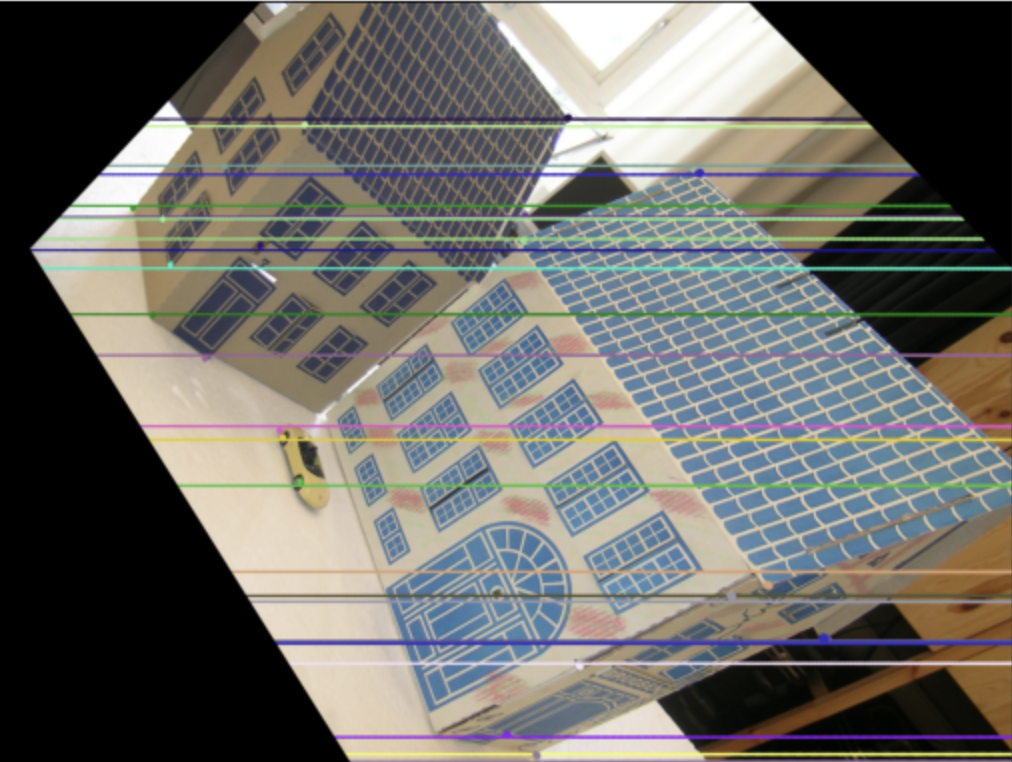
\includegraphics[width=\linewidth]{Materials/BaselineScanlineB}
	\end{subfigure}
	\caption{The baseline estimation brought to scanline agreement.}
	\label{baselineScanline}
\end{figure}
As the 'scanline agreement error' is ambiguous to me, I have chosen to follow the 'rectification error' from \cite{rectificationError} which measures the error by computing the mean and standard deviation of the \textit{y-disparity} between the points in image A and image B after rectification. Here we find a \textbf{mean} of \textbf{8.53} and a \textbf{standard deviation} of \textbf{7.41} which tells us our epipolar lines on average are fairly close to go through our points in the images, but the variance is also fairly high, which implies some of our points are very close, and some are quite far off.